\documentclass[../Article_Model_Parameters.tex]{subfiles}
\graphicspath{{\subfix{../Figures/}}}
\begin{document}
	
	\label{CH: Experiments}
	
	In order to solve the optimization problem presented by Equation \ref{EQ: Optimization_formulation_MLE}, it is necessary to have knowledge of the dataset ${\color{black}Y}(t)$, which was obtained by extracting caraway oil from caraway seeds. To prepare the seeds for extraction, they were first pre-treated using a Retsch SM 300 cutting mill to reduce their particle size to 1mm and break their outer shell. The moisture content of the seeds was then determined using an Infrared Moisture Analyser, which revealed an average moisture content of 4.83\% in the solid particles after grinding. Next, the density of the solid material was measured using a pycnometer, which can be found in Appendix \ref{CH: Solid_Density_Measurment}. Finally, the material's porosity was also calculated to be 0.5, as explained in Appendix \ref{CH: Porosity}.
	
	The caraway seeds used in the experiments were obtained during the 2022 harvesting season. The experiments were conducted using a 10-litre extractor with an inner diameter of approximately 15 cm and a height of 60 cm. Four experiments were performed under different operating conditions: $40~^\circ C$ / 200 bar, $50~^\circ C$ / 200 bar, $40~^\circ C$ / 300 bar, and $50~^\circ C$ / 300 bar. The volumetric flow rate used in all experiments was on average 0.4 litres per minute, with negligible variations (up to 5\%). The amount of solid material used for extraction was 1 kg (or 1.6 litres), which was not enough to fill the entire extraction chamber.
	
	After loading the material into the extraction chamber, the extractor was pre-heated to the desired temperature. The outlet line was then closed, and the extraction chamber was filled with $CO_2$. The $CO_2$ was pumped and compressed until the desired operating pressure was reached. When the operating temperature and pressure were achieved, the outlet line was opened, allowing the solvent to flow through the system. The solvent extracted the essential oils from the solid material, and the resulting $CO_2$ and oil mixture flowed from the extractor to the separator. The separator operated at $50^\circ C$ and $50$ bar. The gaseous $CO_2$ exited from the top and was recycled to the $CO_2$ storage tank. The oil stayed at the bottom of the separator in the liquid form. The extraction time for each batch was 150 minutes, measured from the opening of the extractor outlet port. Every 5 minutes, the oil was drained from the separator, and its weight was measured. The resulting time series ${\color{black}Y}(t)$ corresponds to the output of measurement Equation \ref{Model_measurment_1} and can be used for parameter estimation.
	
	\begin{figure}[!h]
		\centering
		\begin{subfigure}[b]{\columnwidth}
			\centering
			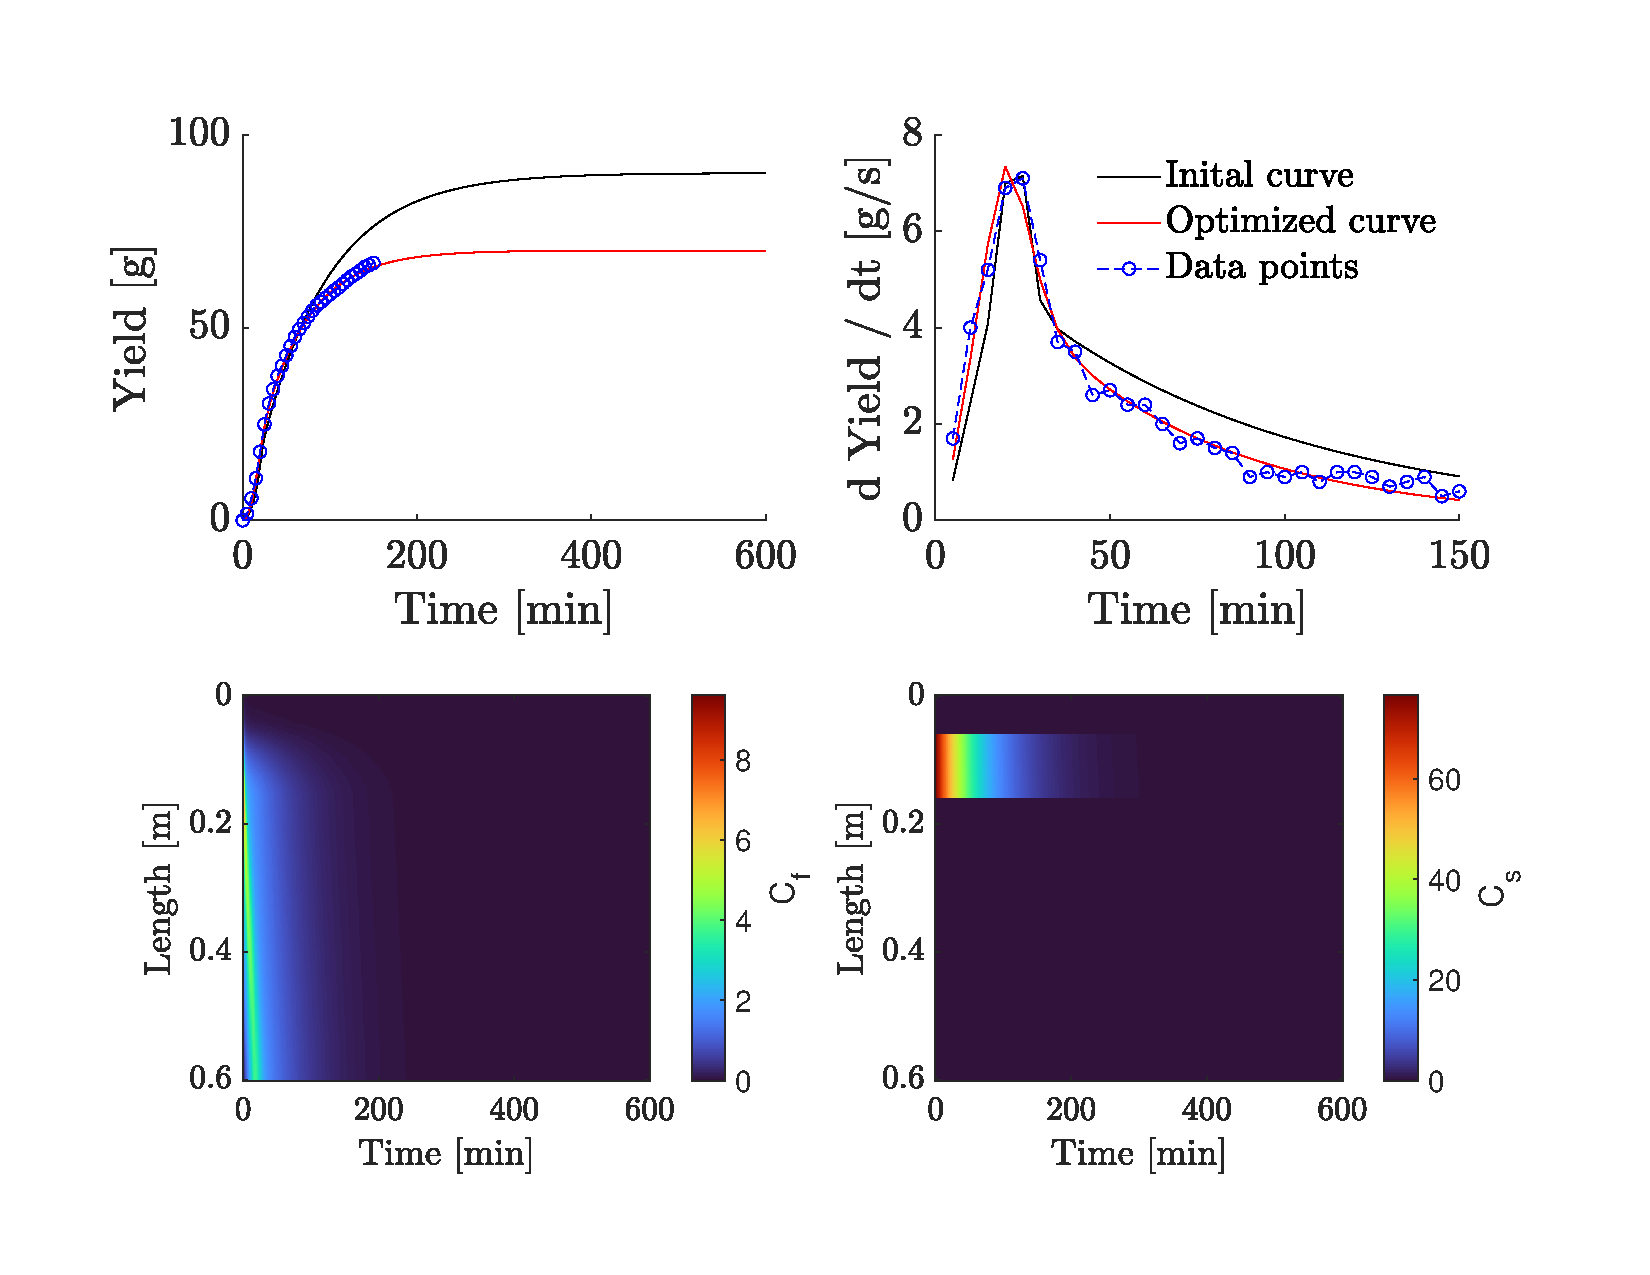
\includegraphics[trim = 2cm 10.5cm 2.5cm 1.7cm,clip,width=0.99\textwidth]{/Results_estimation/Fitting_LUKE_T40_P200.pdf}
			\caption{Experiment at $40~^\circ C$ and 200 bar}
		\end{subfigure}
		\begin{subfigure}[b]{\columnwidth}
			\centering
			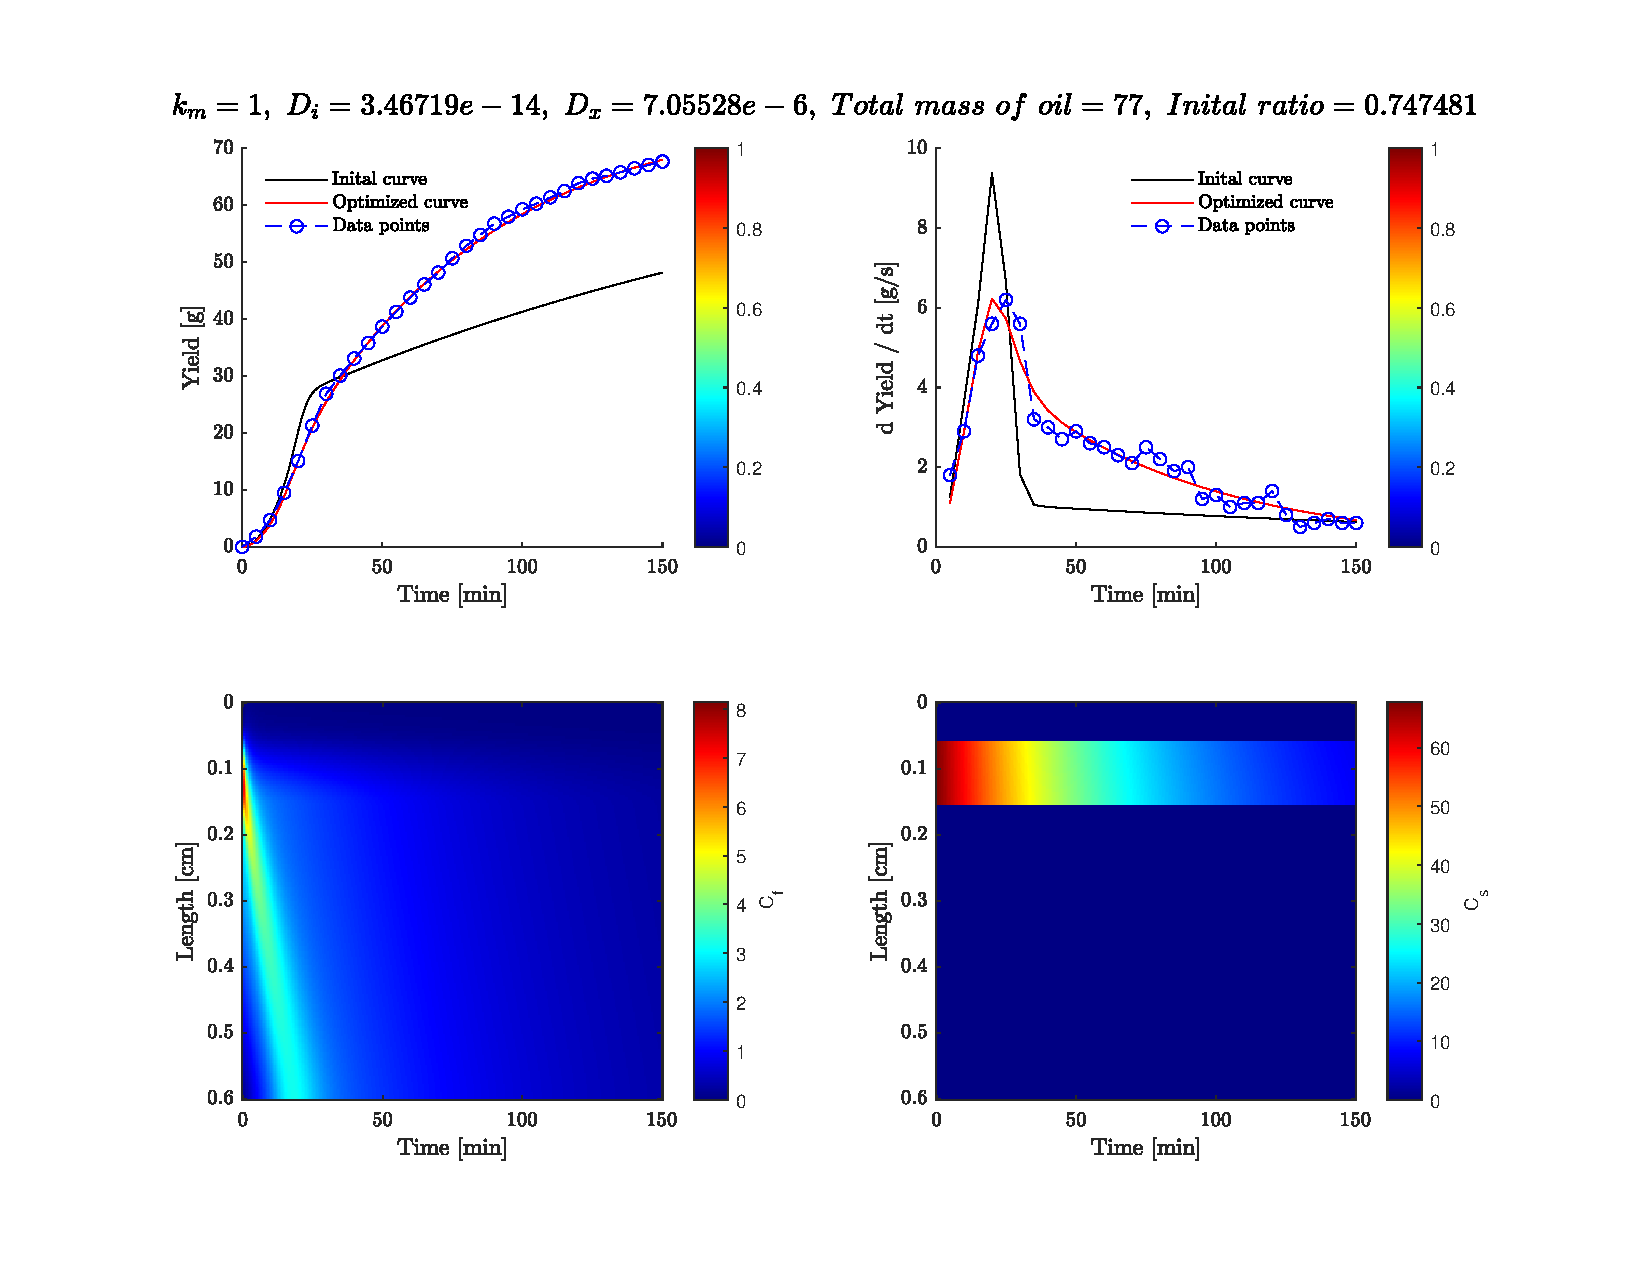
\includegraphics[trim = 2cm 10.5cm 2.5cm 1.7cm,clip,width=0.99\textwidth]{/Results_estimation/Fitting_LUKE_T50_P200.pdf}
			\caption{Experiment at $50~^\circ C$ and 200 bar}
		\end{subfigure}
		\hfill
		\begin{subfigure}[b]{\columnwidth}
			\centering
			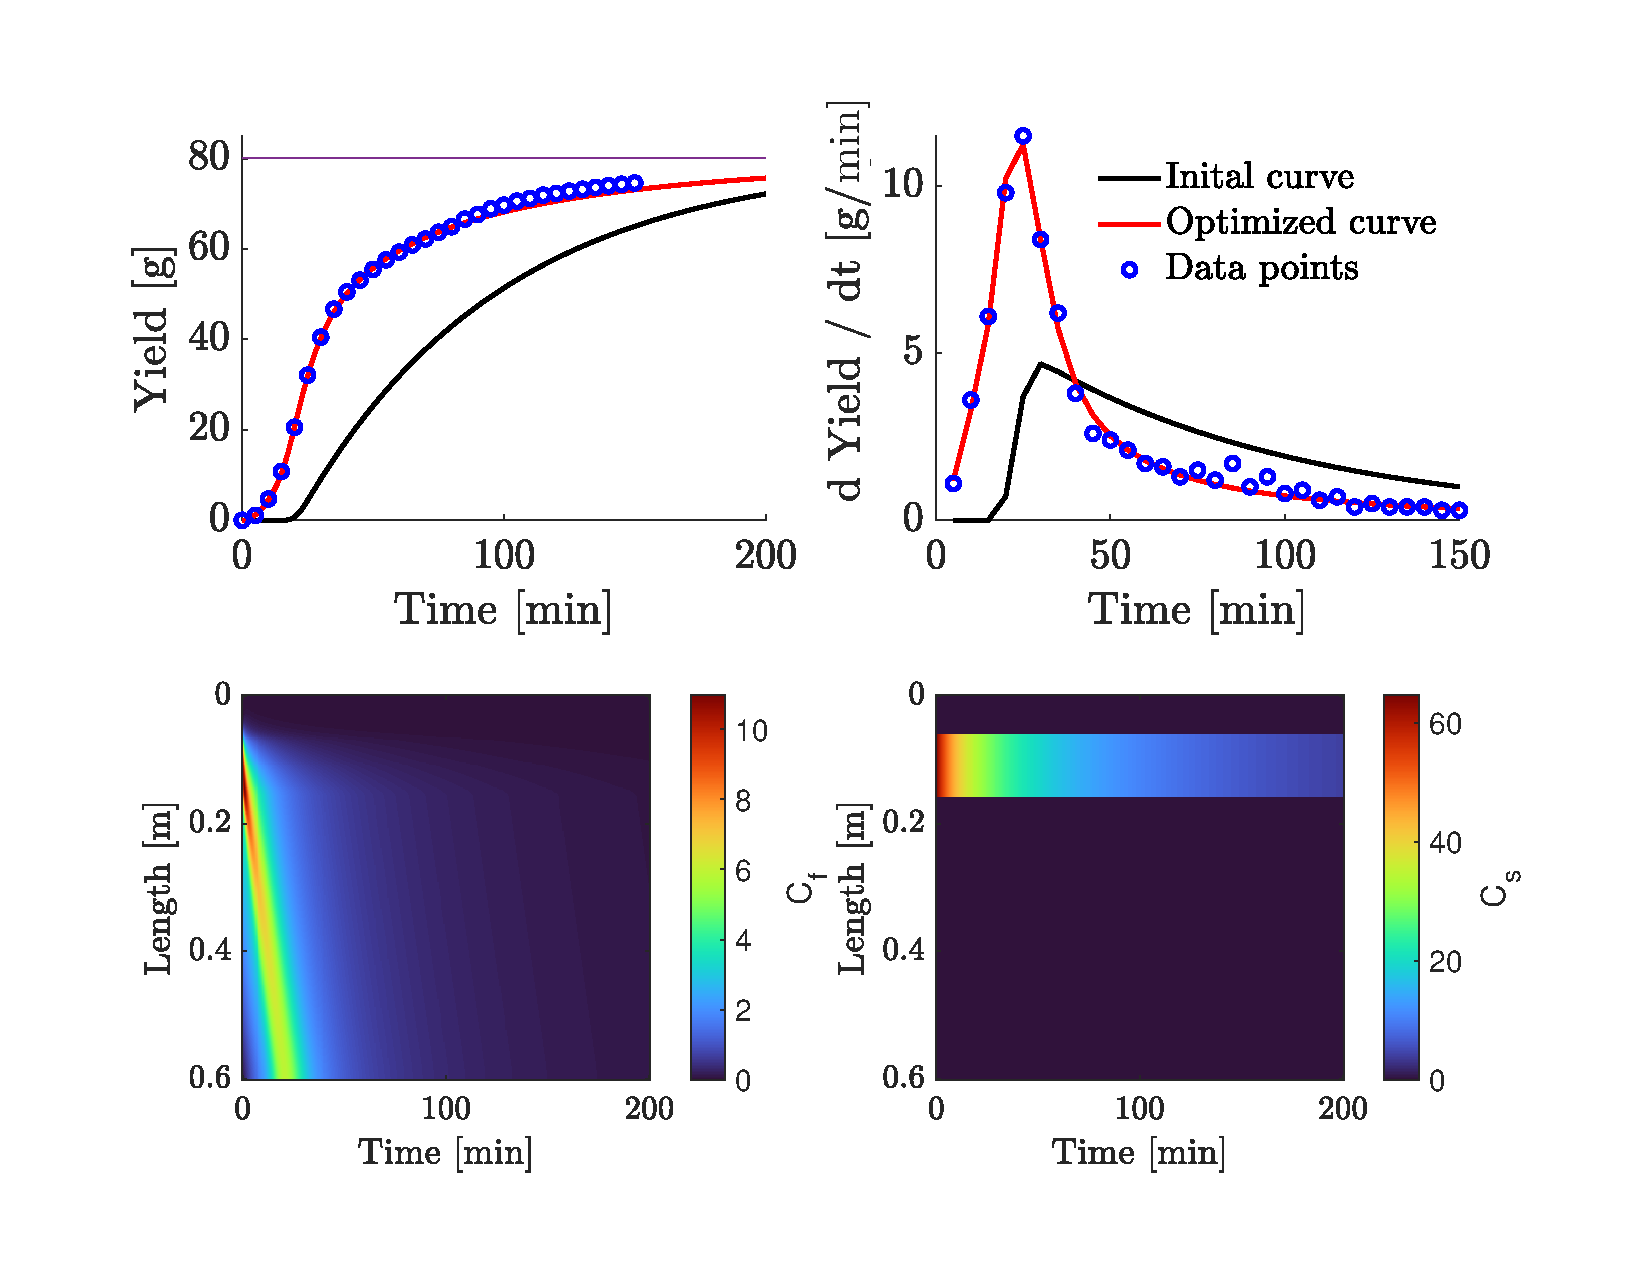
\includegraphics[trim = 2cm 10.5cm 2.5cm 1.7cm,clip,width=0.99\textwidth]{/Results_estimation/Fitting_LUKE_T40_P300.pdf}
			\caption{Experiment at $40~^\circ C$ and 300 bar}
		\end{subfigure}
		\begin{subfigure}[b]{\columnwidth}
			\centering
			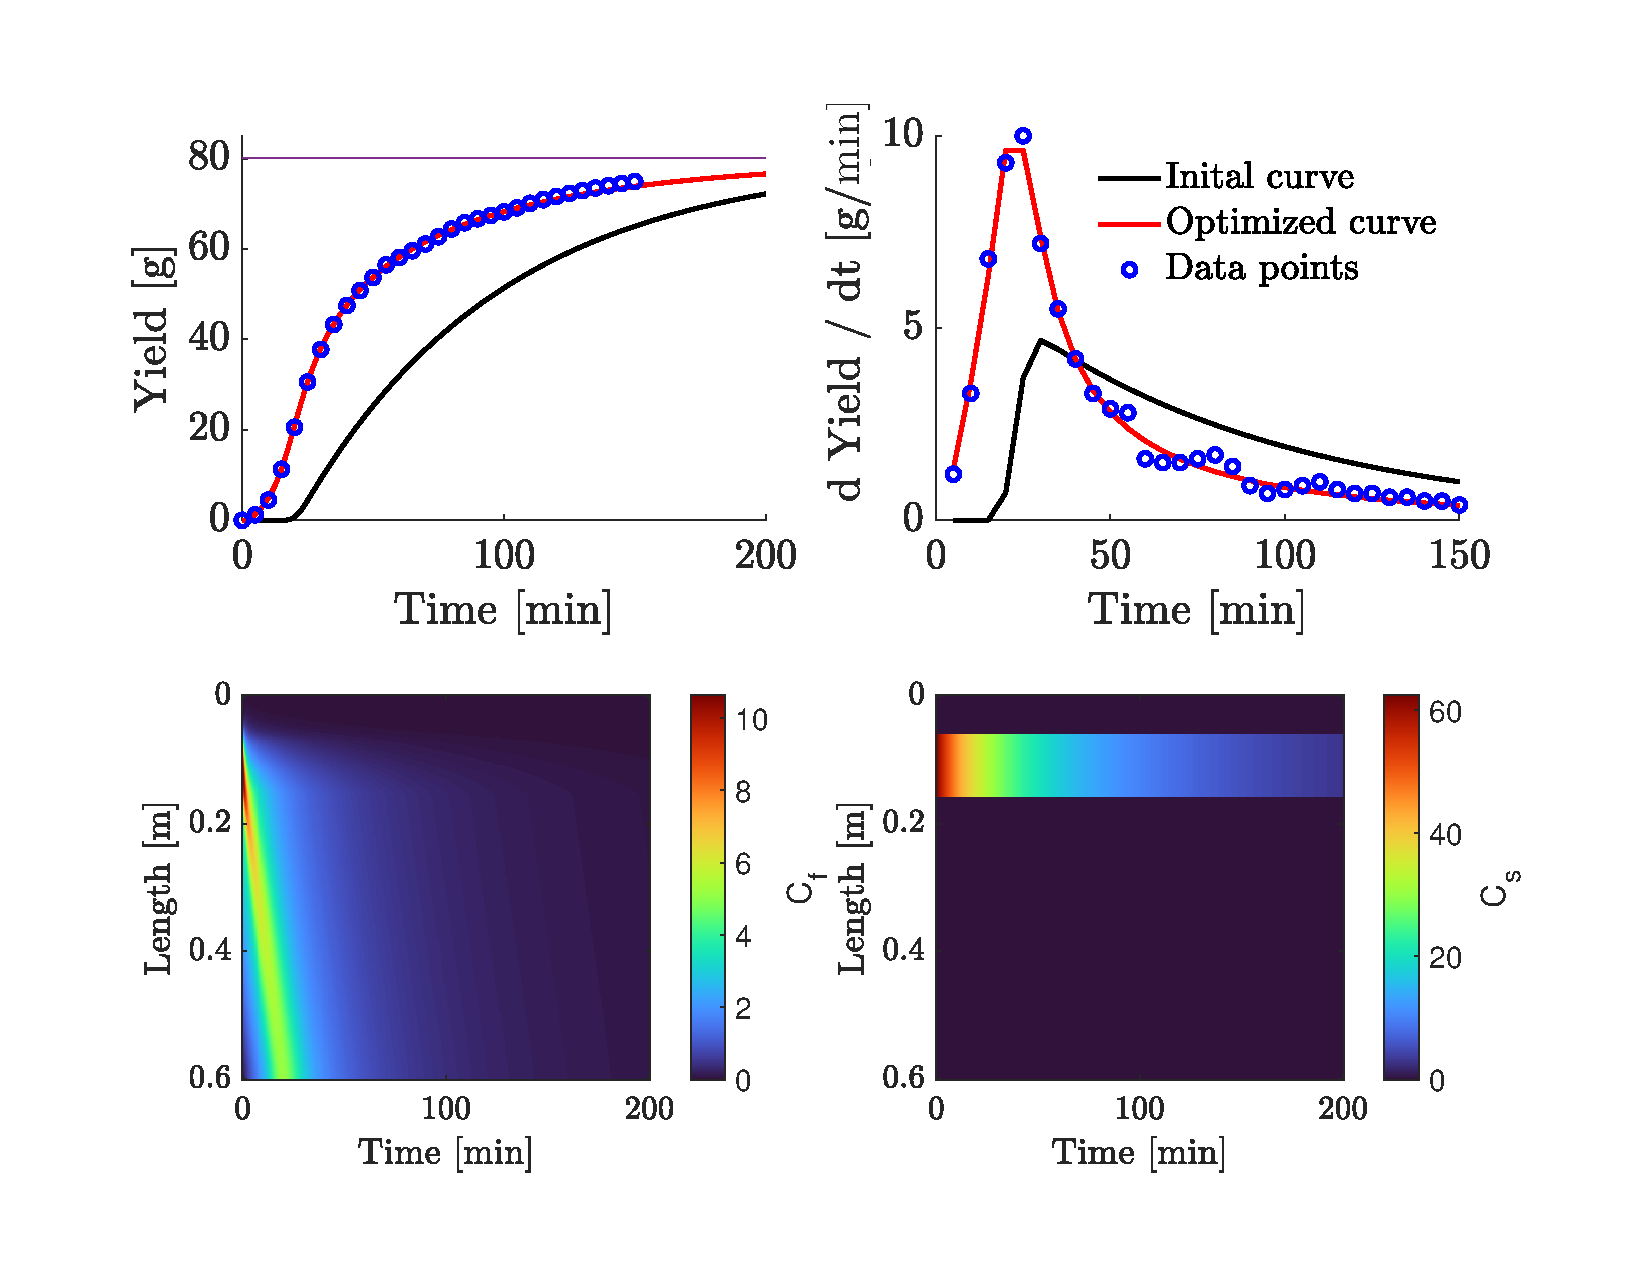
\includegraphics[trim = 2cm 10.5cm 2.5cm 1.7cm,clip,width=0.99\textwidth]{/Results_estimation/Fitting_LUKE_T50_P300.pdf}
			\caption{Experiment at $50~^\circ C$ and 300 bar}
		\end{subfigure}
		\caption{Results of parameter estimation}
		\label{fig: estimation_results}
	\end{figure}
	
\end{document}